\chapter{驱动程序的设计和实现}
	
\section{USB口转串口驱动的设计}

	USB口转串口驱动程序的编写与操作系统的关系密不可分。设备驱动程序在操作系统中如何存在、如何与操作系统的其它部分相联系、如何与操作系统的其他部分相联系、如何为用户提供服务都是操作系统的设计人员在设计操作系统时制定的,系统已经为驱动程序制定好了一个框架,无论驱动程序的开发人员以何种方式控制设备,他们所开发的驱动程序都是以预先设计好的方式存在、与操作系统其他部分相联系和为用户提供服务的\cite{徐媛媛2003嵌入式实时操作系统的设备驱动}。我们此次驱动程序需要实现的框架部分主要包括cp210xDrvInit()、cp210xDevOpen()、cp210xDevClose()、cp210xDevIoctl()、cp210xDevWrite()、cp210xDevRead()、cp210xDrvUnInit()等函数,如\autoref{lab:驱动程序的关键模块}所示 ,以及用于处理数据的缓冲区、用于进行同步和互斥操作的信号量。
\begin{table}[!h]
\centering
\begin{tabular}{|c|c|}
\hline
{模块} & {作用} \\
\hline
{cp210xDrvInit()} & \tabincell{c}{这个模块用来初始化驱动程序,主要是与设备无关的一些\\全局变量并向系统注册该驱动} \\
\hline
{cp210xDevOpen()} & \tabincell{c}{这个模块用来转接I/O子系统分发过来的open()操作,实现设备的打开,\\返回文件描述符} \\
\hline
{cp210xDevClose()} & \tabincell{c}{这个模块用来转接I/O子系统分发过来的close()操作,实现设备的关闭,\\对设备占用资源进行清理} \\
\hline
{cp210xDevIoctl()} & \tabincell{c}{这个模块用来转接I/O子系统分发过来的ioctl()操作,\\实现对设备的一些特定的控制操作} \\
\hline
{cp210xDevWrite()} & \tabincell{c}{这个模块用来转接I/O子系统分发过来的write()操作,\\实现对设备进行数据的写入} \\
\hline
{cp210xDevRead()} & \tabincell{c}{这个模块用来转接I/O子系统分发过来的read()操作,\\用于从设备读取数据。} \\
\hline
{cp210xDrvUnInit()} & \tabincell{c}{这个模块用来卸载驱动程序,将驱动从系统驱动表中删除,\\并清理该驱动程序所占用的全部资源} \\
\hline
\end{tabular} 
\caption{驱动程序的关键模块}\label{lab:驱动程序的关键模块}
\end{table}
	
	另外一个方面,USB口转串口的驱动程序需要硬件来作为支撑,PC机上本身并没有USB/RS-232的转换器,
	对于USB/RS-232转换器的设计通常有两类实现方式:一类是采用全面系统的设计,使用包含有USB单元的微处理器,要求它具有内置的通用异步收发器(UART)在USB和RS-232之间进行信号转换,这样的控制器包括PCI16C745、68HC705JB4和C541U系列等\cite{USB与RS232接口转换器的设计},也可以采用USB接口芯片如PDIUSBD12、USBN9604等与微控制器组合工作;第二类方法是采用专用的USB/RS-232双向转换芯片,如CP2102、FT232BM等,我们在此处的设计即使用了CP2102芯片作为USB/RS-232转换器,这样设计的好处是不需要编写转换器芯片的固件,节约开发时间,由于这个技术已经很成熟,大多的USB口转串口的解决方案都会采用这种已经设计好的集成芯片来作为转换器。我们本次使用的设备如\autoref{fig:cp2102模块正反面}所示。
\begin{figure}[h]
\centering
  \begin{subfigure}[b]{0.4\textwidth}
  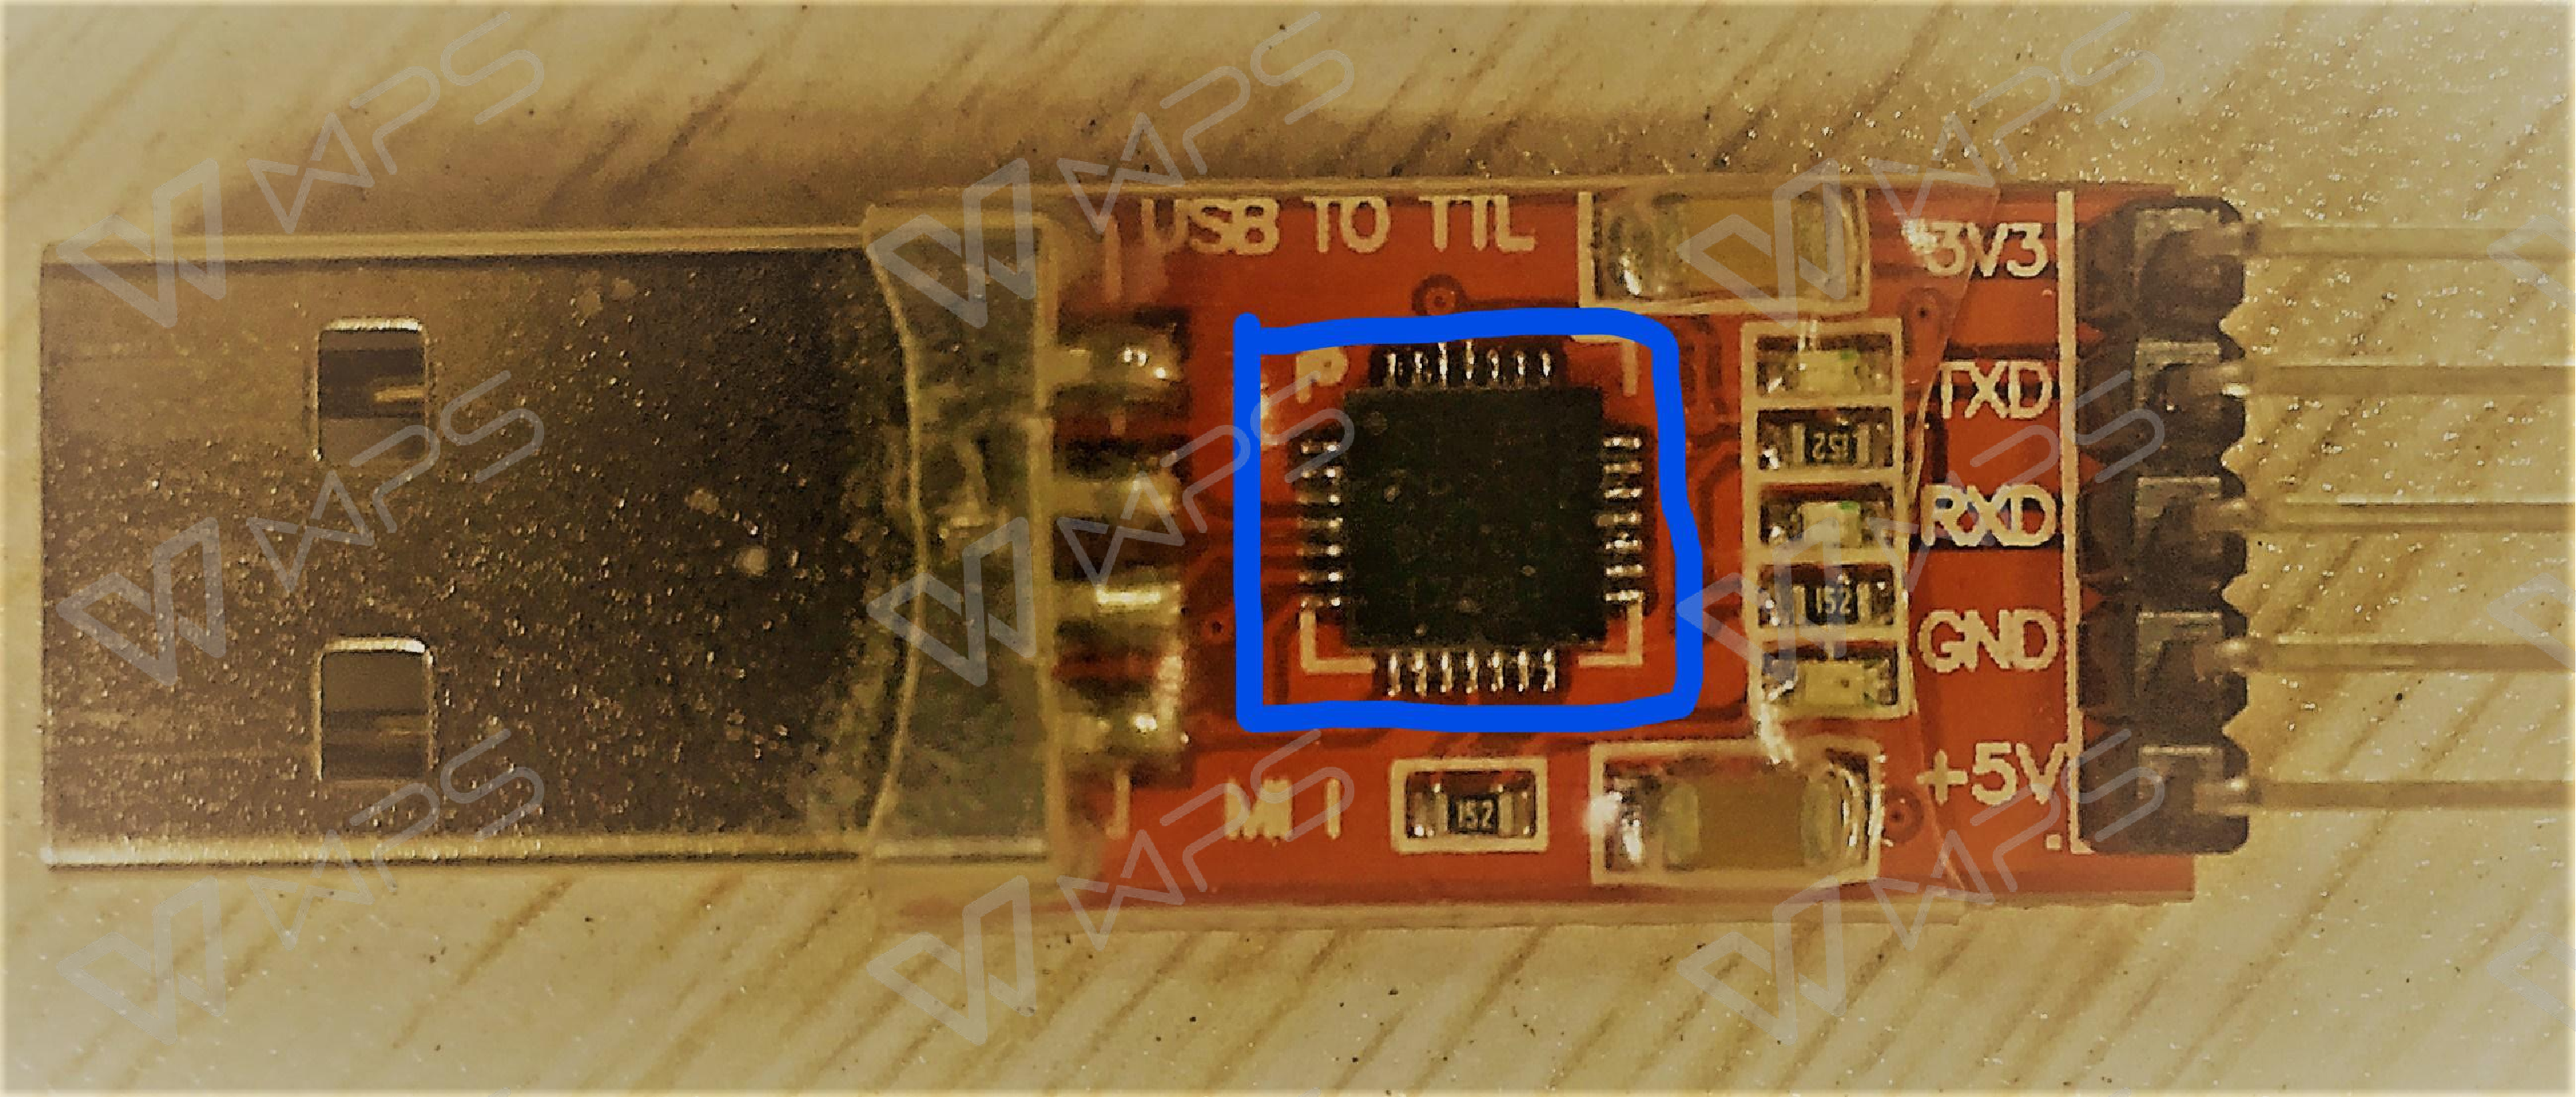
\includegraphics[width=\textwidth]{./graphics/cp2102Front.pdf}
  \caption{CP2102模块正面}\label{fig:cp2102Front}
  \end{subfigure}
  ~
  \begin{subfigure}[b]{0.4\textwidth}
  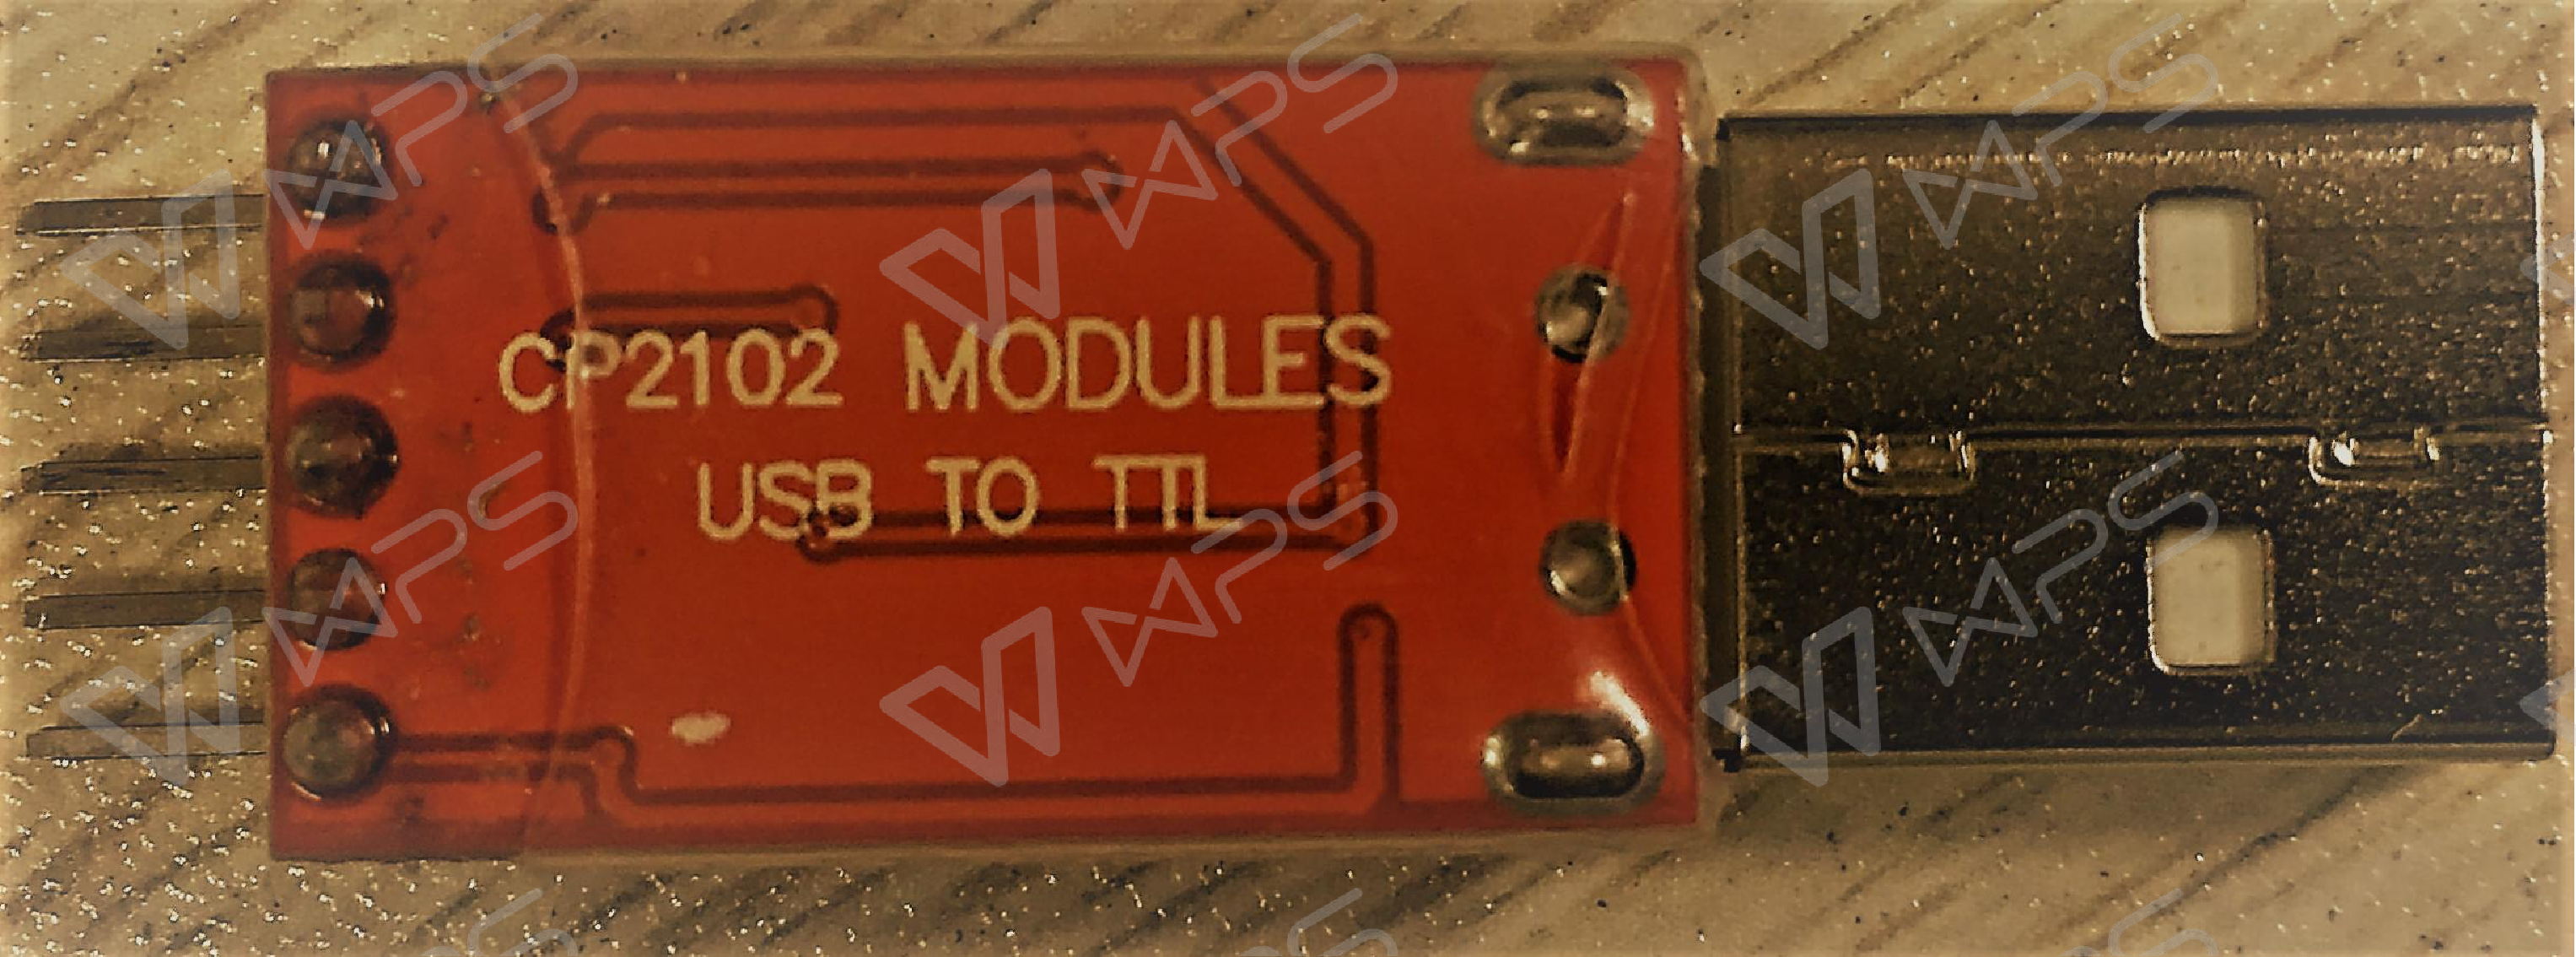
\includegraphics[width=\textwidth]{./graphics/cp2102Rear.pdf}
  \caption{CP2102模块反面}\label{fig:cp2102Rear}
  \end{subfigure}
\caption{CP2102模块正反面}\label{fig:cp2102模块正反面}
\end{figure}




\subsection{CP2102开发}
	
	CP2102是SILICON LABORATORIES推出的USB与RS232接口转换芯片,是一种专门用来进行USB转UART的高度集成的桥接器,和其他同类型的芯片相比具有功耗更低、体积更小、集成度更高(仅需少量外部元件)、价格更低等优点。因此我们此次选择这个芯片作为调通道的设计当中使用的芯片。CP2102提供一个使用最小化的元件和PCB空间实现RS232转USB的简便的解决方案。
	CP2102芯片包含有一个USB2.0全速功能控制器,EEPROM,USB收发器,振荡器和带有全部的调制解调器控制信号的异步串行数据总线(UART),CP2102将全部的部件集成在一个5mm*5mm MLP-28封装的IC当中\cite{CP2102},CP2102的电路框图如\autoref{fig:cp2102电路框图}所示。

\begin{figure}[!h]
\centering
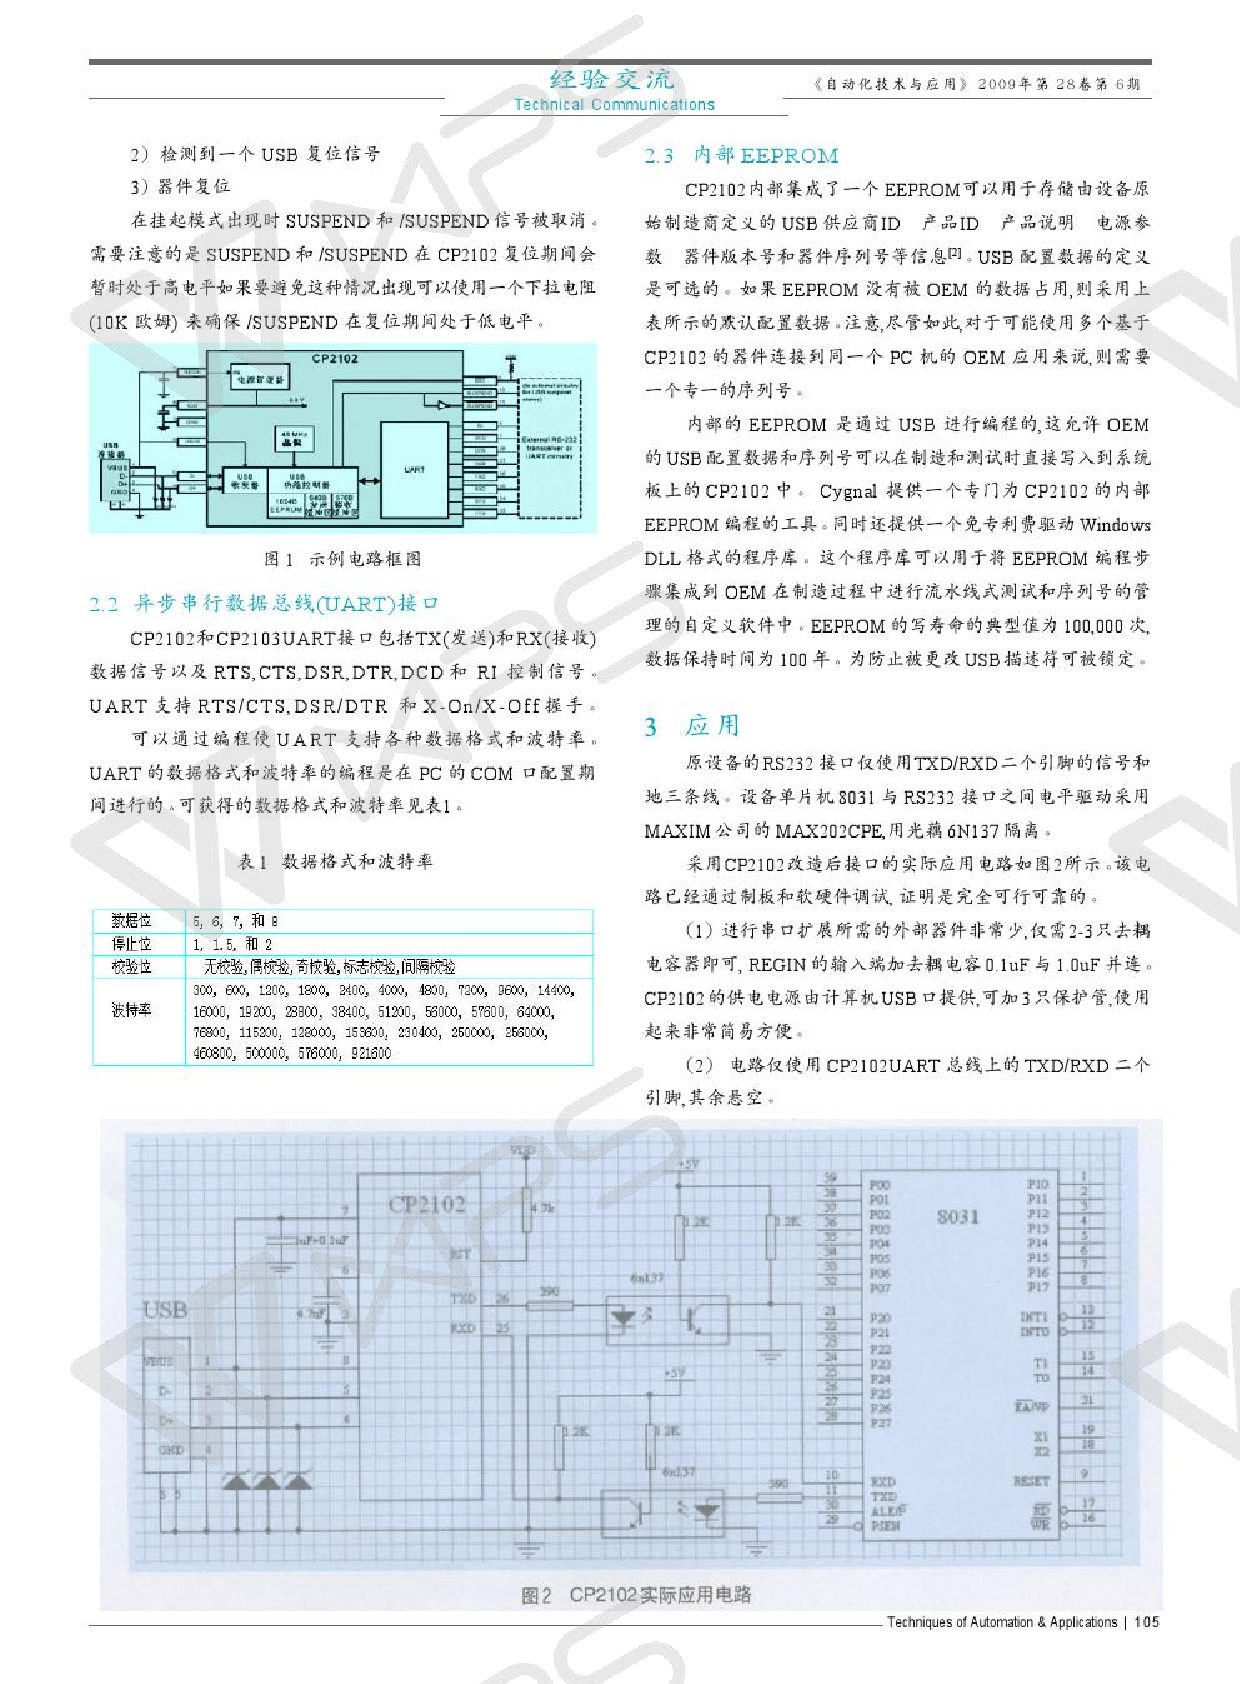
\includegraphics[width=1.0\textwidth]{./graphics/cp2102-circuit-diagram.pdf}
\caption{cp2102电路框图}\label{fig:cp2102电路框图}
\end{figure}

	使用CP2102进行串口扩展的时候所需要的外部器件是非常少的,仅仅需要2-3个去耦电容即可,在SILICON给出的文档当中已经帮我们给出了一个最简单的连接电路图,如\autoref{fig:cp2102电路框图}所示。电路使用CP2102UART总线上的TXD/RXD两个引脚,其余的引脚都悬空。CP2102可以完成USB/RS-232双向转换(需要外接一个TTL电平到RS-232电平的芯片),一方面可以从主机接收USB数据并将其转换为RS232信息格式流发送给外设,另外一方面可以从RS232外设接收数据转换为USB数据格式传送回主机。使用时我们只需要将数据通过USB的数据包发送给CP2102芯片即可,芯片会自动进行解析和控制。
		
\begin{enumerate}
\item CP2102的USB功能控制器和收发器:CP2102的USB功能控制器是一个符合USB2.0协议的全速器件,这个器件负责管理USB和UART之间的所有数据传输以及由USB主控制器发出的命令请求和用于控制UART功能的命令。
\item 异步串行数据总线(UART)接口:CP2102的UART接口包括TXD(发送)和RXD(接收)数据信号以及RTS,CTS,DSR,DTR,DCD和RI控制信号。ART支持RTS/CTS,DSR/DTR和X-on/X-Off握手。且支持编程使UART支持各种数据格式和波特率。ART的数据格式和波特率的编程是在PC的COM口配置期间进行的。可以使用的数据格式和波特率见\autoref{CP2102可配置参数}。
\item 内部EEPROM:CP2102内部集成了一个EEPROM用于存储设备原始制造商定义的USB供应商ID、产品ID、产品说明、电源参数、器件版本号和器件序列号等信息\cite{CP2102}。USB配置数据的定义是可选的,如果EEPROM没有被OEM的数据所填充的话,则设备会自动的使用一组默认的数据如\autoref{CP2102DefaultConfigure}所示。
\end{enumerate}

\begin{table}[!h]
\centering
\begin{tabular}{|c|c|}
\hline
{数据位} & {5,6,7,8} \\
\hline
{停止位} & {1,1.5,2} \\
\hline
{校验位} & {无校验,偶校验,奇校验,标志校验,间隔校验} \\
\hline
{波特率} & \tabincell{c}{600,1200,2400,4800,7200,9600,14400,16000,19200,28800,\\ 38400,51200,56000,57600,64000,76800,115200,128000,158600,\\ 230400,250000,256000,4608000,576000,921600}\\
\hline
\end{tabular} 
\caption{CP2102可配置参数}\label{CP2102可配置参数}
\end{table}

\begin{table}[!h]
\centering
\begin{tabular}{|c|c|}
\hline
{\hei{Name}} & {\hei{Value}} \\
\hline
{Vendor ID} & {10C4h} \\
\hline
{Product ID} & {EA60h} \\
\hline
{Power Descriptor(attributes)} & \tabincell{c}{80h}\\
\hline 
{Power Descriptor(Max Power)} & {32h} \\
\hline
{Release Number} & {0100h} \\
\hline
{Serial Number} & {0001(63 characters maximum)} \\
\hline
{Product Description String} & \tabincell{c}{"CP2102 USB to UART Bridge Controller”(126 characters maximum)"} \\
\hline
\end{tabular}
\caption{CP2102默认配置表}\label{CP2102DefaultConfigure}
\end{table}
	
	CP2102当中的协议控制单元会通过接受USB接口的命令,对UART接口进行配置(如配置通信的波特率、数据位、校验位、起始/停止位、流控信号等)。CP2102当中的接收和发送缓冲区用来临时保存双方在数据传输过程中的数据。以从计算机到外设的数据传输为例。当USB转串口设备连接到PC的USB总线上时,PC在检测到设备连接之后会对设备进行初始化并启动相关的客户端驱动程序;之后会由驱动程序给设备发送配置命令,设置设备的数据传输特性;最后,在数据传输的时候,计算机上的驱动程序会将数据包传输给USB接口(通常使用批量传输的方式),设备从USB接口提取出数据并保存在数据缓冲区中,UART接口再从数据缓冲区中将数据取走并发送出去,从外设传输数据到计算机的方式则相反。





\subsection{VxWorks上的USB开发}
	VxWorks 的I/O框架由ioLib.c 文件提供,但ioLib.c文件提供的函数仅仅是一个最上层的接口,并不能完成具体的用户请求,而是将请求进一步向其他内核模块进行传递,位于ioLib.c模块之下的模块就是iosLib.c。我们将ioLib.c 文件称为上层接口子系统,将iosLib.c文件称为I/O 子系统,注意二者的区别。上层接口子系统直接对用户层可见,而I/O 子系统则一般不可见(当然用户也可以直接调用iosLib.c 中定义的函数,但一般需要做更多的封装,且违背了内核提供的服务层次),其作为上层接口子系统与下层驱动系统的中间层而存在。VxWorks的内核驱动层次结构如\autoref{fig:VxWorks内核驱动层次结构}所示。

\begin{figure}[!h]
\centering
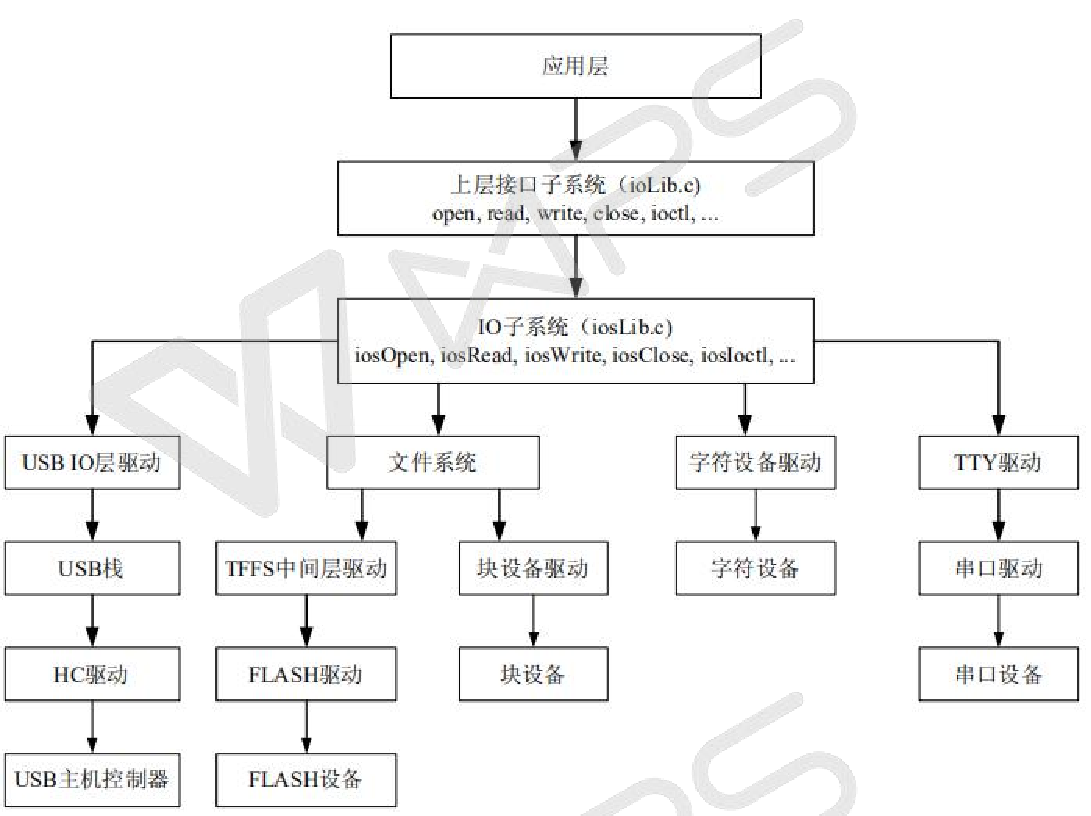
\includegraphics[width=0.9\textwidth]{./graphics/vxworks-kernel-diagram.pdf}
\caption{VxWorks驱动内核层次结构}\label{fig:VxWorks内核驱动层次结构}
\end{figure}	
			
	VxWorks的USB主机驱动程序堆栈满足USB协议规定的要求,提供了一整套服务来操作USB以及一些预置USB类驱动程序,以处理特定类型的USB设备。在Wind River的VxWorks中USB驱动程序堆栈的开发符合的是通用串行总线规范2.0版,USB系统是一种主从结构,系统的所有动作都是由USB主机发起,并协调不同的设备动作,设备端软件在系统中只需要对主机的命令做出响应即可,USB的主机端由于在系统中的地位比较特殊,因而其软件结构比较复杂,USB协议在主机端是分层实现的,其通信的逻辑结构和PC端的软硬件结构如\autoref{fig:usb通信结构}所示。USB协议由上至下可以分为三层:客户端驱动程序(Client Driver)、USB驱动(USBD)、主机控制器驱动(HCD),每一层完成不同的功能。

\begin{figure}[h]
\centering
  \begin{subfigure}[b]{0.4\textwidth}
  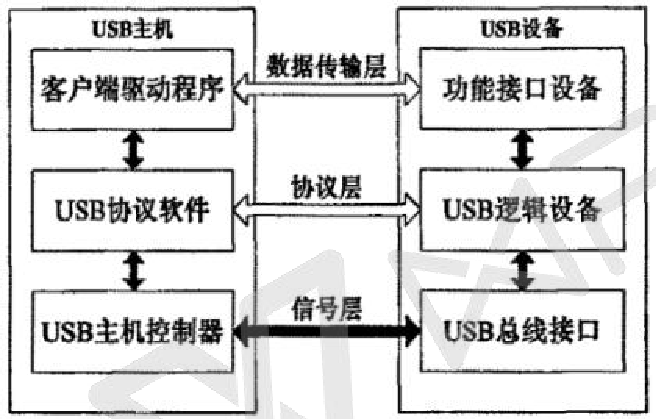
\includegraphics[width=1.0\textwidth]{./graphics/USB-device-structure-diagram.pdf}
  \caption{USB通信的逻辑结构}\label{fig:usb通信逻辑结构}
  \end{subfigure}
  ~
  \begin{subfigure}[b]{0.5\textwidth}
  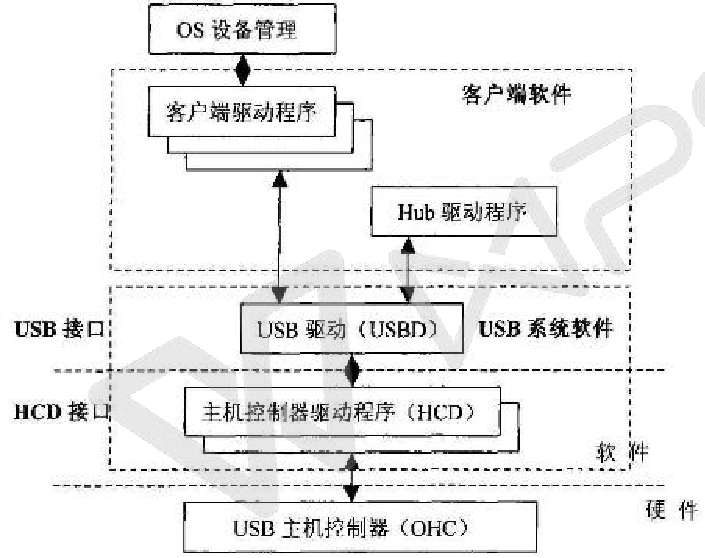
\includegraphics[width=1.0\textwidth]{./graphics/USB-PC-structure.pdf}
  \caption{USB主机端软硬件结构}\label{fig:usb-PC}
  \end{subfigure}
\caption{USB通信结构}\label{fig:USB通信结构}
\end{figure}
	
	客户端驱动程序完成对不同的设备类的设备的功能驱动。本次设计中所要完成的USB口转串口的驱动要完成的就是客户端驱动。为了和设备进行正常的通信,他通过USB的I/O请求包(I/O request,IRP)向USBD层发出数据接收或者发送的请求。此外,USB的传输机制对于客户端的驱动程序而言是完全透明的,客户端驱动程序所看到的仅仅是具体的设备类,不管设备采用的何种的数据传输方式。另外IRP是USB协议定义的抽象概念,其结构需要根据协议的具体来实现。
	
	USBD是USB的核心驱动,其提供的功能包括USB总线的枚举、总线带宽的分配、传输控制等操作。向上的接口负责处理客户端驱动程序提出的I/O请求,他通过IRP了解此设备的属性和本次数据通信的具体要求,将此IRP转换成USB能够识别的一系列的事物处理,交给HCD层或直接交给主机控制器处理。USBD还负责新设备的动态插拔、USB电源管理和对客户端驱动程序的维护等操作。
	
	HCD层的主要功能是与主机控制器合作完成USB的各种事物处理。它根据一定的规则调度所有奖杯广播发送到USB上的事物处理。调度方法是首先将数据传输类型组成不同的链表,每一种链表包括来自不同的设备驱动程序的同一种类型的数据,然后定义不同的数据类型在传输中所占的带宽比例,交给主机控制器处理,控制器根据规则从立案表上摘下数据块,根据大小为它创建一个或者多个事物处理,完成与设备的数据传输,当事物处理完成时HCD将结果交给USBD层。此外它还完成对主机控制器和根集线器的配置和驱动等操作。WindRiver提供了两种类型的主机控制器驱动:usbHcdUhciLib(UHCI主机控制器驱动)和usbHcdOhciLib(OHCI主机控制器驱动)。VxWorks的USBD和HCD之间的接口允许操过一个的底层主控制器,并且USBD能够同时连接多个USB HCD。这样的设计特点可以让开发者建立复杂的USB系统。
	
	在VxWorks系统当中UBSD层的驱动和HCD层的驱动都是已经实现好的,我们所需要实现的是客户端的驱动程序,用以驱动特定的USB设备。典型的USB设备的描述符一般由USB标准描述符和USB类描述符组成,或者由USB标准描述符和USB厂商特定描述符组成。任何一个USB设备都必须包含USB标准描述符,他提供了设备的基本信息和通信方式。为了简化USB设备的开发过程,通常会将具有相同的或者是相识的功能的设备归为一类,并指定相关的类规范,这样就能够保证只要按照同样的规范标准,即使是不同的厂商开发的USB设备也能够使用相同的驱动程序。针对不同类型的USB设备,USB-IF规定了相关的类描述符,他在标准描述符的基础上进一步说明了特定类型的设备共能以及相关的数据传输方式。但是USB-IF规定的设备类描述符并不能够覆盖所有的电子设备,对于没有相关的类描述符的USB接口,生产厂商需要利用自己提供的厂商特定功能的类描述符和设备命令对其通信特性做出说明,这些特定功能的描述符和命令的定义和操作完全取决于厂商,要想驱动此类设备就必须要参考厂商提供的这些专有命令。CP2102模块就属于这种没有相关的类描述符的设备,他不但支持USB的标准描述符和USB标准命令,还支持自己特定的描述符和命令,我们称这样的设备为非标准类型的USB设备。非标准的设备命令和描述符的结构和处理方式与标准设备命令和描述符是一样的,但是它只对特定的功能设备有效。

	
	


\subsection{环形缓冲区的设计}
	在我们的USB口转串口驱动程序当中 ,我们需要解决低速设备和处理器之间、USB接口和RS-232串口之间的速度匹配问题 ,如果每次数据传送或接收时系统任务都去操作数据 ,这样必会造成任务频繁切换 ,系统效率降低。解决办法之一就是在设备驱动和应用程序之间建立环形数据缓冲 ,当数据到达时 ,系统会产生中断 ,USBD层会处理中断,然后调用我们注册的输入IRP来处理数据,将接受的数据放到我们设计的缓冲中 ,应用程序在需要接收数据时 ,从环形缓冲中的另一端(即最先放入数据的一端)读取数据,是一种先进先出缓冲结构。
		
	
  应用程序、设备驱动和环形缓冲区的关系如\autoref{fig:设备数据缓冲}所示,通过环形数据缓冲,我们可以解决速度匹配的问题,大大降低系统的开销。
	我们使用循环队列实现的来实现缓冲区,并设置对头指针和队尾指针,其特点是当一个数据元素被取走以后,其余的数据元素不需要移动其存储位置。在设备初始化时,将设备的环形缓冲区清空,队头指针和队尾指针均设为 0,之后通过操作队头指针与队尾指针来填充数据、移除数据。当驱动中接收到一个数据时,将此数据保存到当前位置 tail++,
	缓冲区当中需要考虑的关键问题是缓冲区的满和空的判断,因为缓冲区满或者是空都有可能出现读指针或者是写指针指向同一个位置。 使用一个空存储单元,在缓冲区中总是使一个存储单元保存为未使用的状态。即一个大小为N的缓冲区中最多只能够存入N-1个数据。如果读写指针指向同一个位置那么缓冲区即为空。如果写指针位于读指针的相邻后一个位置,那么缓冲区为满。在测试缓冲区是否满时做取余运算。在缓冲区已满但还是有数据需要写入的时候,此时我们选择的策略是将最开始的数据进行覆盖,这样操作的好处是可以防止最新的数据丢失,而老的数据可能已经失去了时效性。

\begin{figure}[!h]
\centering
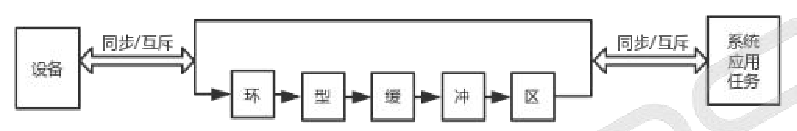
\includegraphics[width=.9\textwidth]{./graphics/Dev-Data-Buf.pdf}
\caption{设备数据缓冲}\label{fig:设备数据缓冲}
\end{figure}


\section{USB转串口驱动的实现}
	在VxWorks中驱动程序对上需要匹配操作系统提供的一套规范接口,对下必须驱动硬件设备进行工作,其起着一个关键的中间转换角色,将操作系统的具体请求转换为对硬件的某种操作,让所有的硬件对操作系统的一套内部规范接口进行响应,屏蔽了硬件的所有复杂性,应用层对于某个设备的操作通过操作系统提供的一套标准接口完成,操作系统最终将这些操作请求传递给驱动程序,驱动硬件完成这些请求。	
	VxWorks调试通道当中运行的最主要的软件平台是嵌入式实时操作系统VxWorks,作为系统的最底层的软件,要想进行数据的传输,驱动程序是必不可少的。本系统中的硬件设备是基于USB总线的,USB口转串口设备的驱动程序在Windows和Linux下都有现成可用的,但是在VxWorks下需要自己来实现这部分。
	
	在VxWorks I/ O 当中通常应该经过以下的三个基本步骤来实现一个设备驱动:
\begin{enumerate}
\item 实现对实际物理设备的数据结构抽象(即设备的自定义数据结构);
\item 完成 I/ O 系统所需要的各类接口及自身的特殊接口(open、read、write等);
\item 将驱动集成到操作系统中。
\end{enumerate}

\subsection{特定需求单设备驱动的实现}

	由于对于仅支持单设备驱动程序是基于特定的需求而具体定制的,所以该设备的驱动程序的实现流程与通常的支持多设备的驱动的初始化流程存在差异。具体的需求为:\\
\hei{1. 驱动中支持的设备名是固定的,无论具体的设备是否连接上,都可以往这个设备中写入数据。}\\
\hei{2. 驱动程序中要有缓存一定数据的能力,一旦设备连接之后就能够检查缓冲区中是否有数据,有数据则将其发送出去。}

	由于需要在设备未连接时就能够往设备中写入数据,且设备名为固定的,那么就必须调整驱动的初始化流程,使得其能够支持这一特性,通常驱动都是在设备加载之后再将其加入到系统设备表和系统驱动表当中,那么此时我们就需要先将一个固定的设备名加入到系统设备表当中。对于该特定需求的单设备驱动的流程图如\autoref{fig:SDev-Drv-diagram}和所示。
\begin{figure}[h]
\centering
  \begin{subfigure}[b]{1.0\textwidth}
  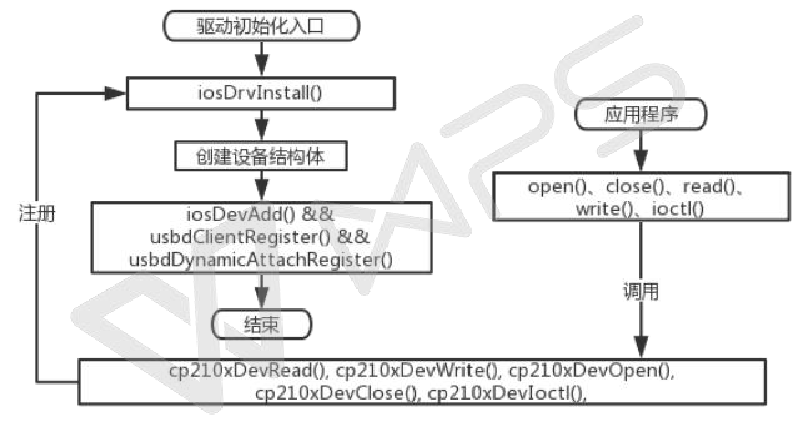
\includegraphics[width=\textwidth]{./graphics/SDev-Drv-Diagram-a.pdf}
  \caption{}\label{fig:SDevice-Driver-diagram-a}
  \end{subfigure}
  ~
  \begin{subfigure}[b]{1.0\textwidth}
  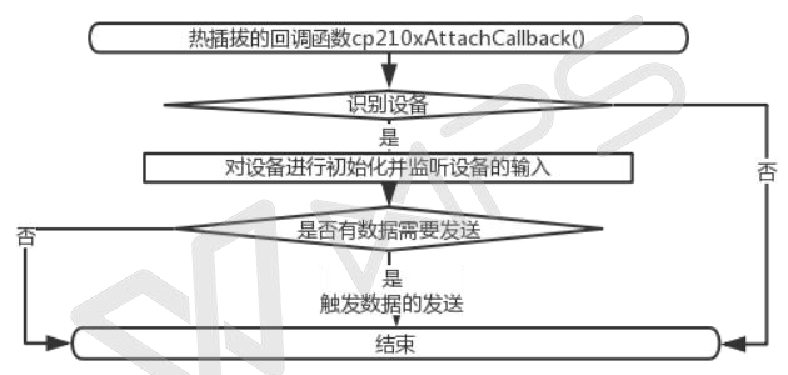
\includegraphics[width=\textwidth]{./graphics/SDev-Drv-Diagram-b.pdf}
  \caption{}\label{fig:SDevice-Driver-diagram-b}
  \end{subfigure}
\caption{特定需求单设备驱动运行流程图}\label{fig:SDev-Drv-diagram}
\end{figure}




\subsubsection{设备的自定义结构}
	底层驱动都要对其驱动的设备维护一个结构,用以保存设备的关键参数:USB配置、接口、端点地址、读写缓冲区的指针等等,这些信息将随着设备类型的不同而有所差别。对于我们此处要驱动的USB口转串口驱动,我们驱动中的关键数据结构如下: 
	
\lstset{language=C}
\begin{lstlisting}
typedef struct cp210x_dev
{
  DEV_HDR cp210xDevHdr;
  
  UINT16 numOpen;
  USBD_NODE_ID nodeId;/*device nodeID*/
  UINT16 configuration;	
  UINT16 interface; /*a interface of this device*/
  UINT16 interfaceAltSetting;
  UINT16 vendorId;
  UINT16 productId;

  BOOL connected;  
  int trans_len;
  USBD_PIPE_HANDLE outPipeHandle; /*USBD pipe handle for bulk OUT pipe*/
  USB_IRP	outIrp; /*IRP to monitor output to device*/
  BOOL outIrpInUse; /*TRUE while IRP is outstanding*/
  UINT16  outEpAddr;
  UINT8 trans_buf[64];

  USBD_PIPE_HANDLE inPipeHandle;/*USBD pipe handle for bulk IN pipe*/
  USB_IRP inIrp;
  BOOL inIrpInUse;
  UINT8 inBuf[64];
  UINT16 	inEpAddr;
} CP210X_DEV, *pCP210XDEV;
\end{lstlisting}
\noindent 部分成员的含义如下:

\begin{itemize}
\item DEV\_ HDR:自定义设备结构的第一个成员必须是DEV\_ HDR结构类型,对于内核的I/O子系统而言,其将所有的设备结构都看作是DEV\_ HDR类型,内核仅仅对DEV\_ HDR结构进行管理,在系统的设备列表中,内核只使用DEV\_ HDR结构当中的成员。自定义结构中的其他成员由驱动自己使用,内核并不了解这些自定义成员。
内核提供这个结构存储一些设备的关键信息,包括链接指针(用以将该结构串入队列中)、驱动索引号、设备节点名。底层驱动需要对其驱动的设备维护一个自定义的数据结构,该结构中包含了被驱动设备寄存器基地址,中断号,可能的数据缓冲区,保存内核回调函数的指针,以及一些标志位。且DEV\_ HDR 内核结构必须是这个自定义数据结构的第一个成员变量,因为这个用户自定义结构最后需要添加到系统设备队列中,故必须能够在用户自定义结构与 DEV\_ HDR 结构之间进行转换,而将 DEV\_ HDR 结构设置为用户自定义结构的第一个成员变量就可以达到这个目的。
\item numOpen:用来记录设备被打开的次数,每次调用open()函数打开该设备则numOpen加一,调用close()函数关闭设备则减一。
\item nodeId:用来保存该设备在系统中的唯一ID号。
\item configure、interface、interfaceAltsetting:用来保存设备的描述符中的配置、接口、可变接口信息。
\item vendorId、productId:保存该设备的厂商ID和产品ID,用来识别该设备是否适合我们的驱动程序。
\item outPipeHandle、inPipeHandle:设备的输入/输出端点的管道句柄,每次传输数据时都需要使用该句柄来表明数据传到的哪一个端点。
\end{itemize}






\subsubsection{驱动注册和设备创建} 
	
	底层驱动一般提供形如 xxxDrv 和 xxxDevCreate 之类的函数完成驱动注册和设备创建的工作。这些工作的完成一般是在内核启动过程中进行。对于此处的USB口转串口驱动我们定义cp210xDrvInit() 初始化函数,其主要完成驱动所需要的资源申请和系统的初始化,包括创建信号量、向系统注册驱动、创建设备、向USBD层注册。cp210xDevInit模块主要代码如下所示:
\lstset{language=C}
\begin{lstlisting}
STATUS cp210xDrvInit(void)
{
  ...
  if(OSS_MUTEX_CREATE(&cp210xWriteMutex) != OK || OSS_MUTEX_CREATE(&cp210xReadMutex) != OK || OSS_MUTEX_CREATE(&cp210xMutex) != OK || (blockReadSem = semBCreate(SEM_Q_FIFO, SEM_EMPTY)) == NULL )
  ... 	
  cp210xDrvNum = iosDrvInstall(NULL,NULL,cp210xDevOpen,cp210xDevClose,
			cp210xDevRead,cp210xDevWrite,cp210xDevIoctl);
  ...
  if( iosDevAdd(&pCp210xDev->cp210xDevHdr,CP210X_NAME,cp210xDrvNum) != OK)
  ...  
  if(usbdClientRegister (CP210X_CLIENT_NAME, &cp210xHandle) != OK)
  ...  
  if(usbdDynamicAttachRegister(cp210xHandle,USBD_NOTIFY_ALL,USBD_NOTIFY_ALL,USBD_NOTIFY_ALL,TRUE,(USBD_ATTACH_CALLBACK)cp210xAttachCallback)!= OK)
  ...
}
\end{lstlisting}\\

	驱动会在进入初始化的时候首先检查该驱动是否已经安装,若已经安装了则无需再次安装,直接退出即可,cp210xDrvInit()通常是在usrRoot(usrConfig.c)中调用,但是你也可以手动调用这个函数对该驱动进行初始化操作。然后会进行一些驱动所需要的全局资源的初始化,如信号量、全局变量、看门狗等,接着调用iosDrvInstall()函数安装驱动的I/O函数,将其添加到驱动表当中,在我们的USB口转串口驱动当中不需要实现delete函数和create函数,直接将其指针置为NULL即可。
	
	注册完成之后还要向系统将该驱动程序添加到IO子系统当中,添加成功后会在系统的设备列表中显示该命名为CP210X\_ NAME的设备(CP210X\_ NAME只是一个宏定义,设备名可以自己更改)。此处即是我们的驱动程序中的一个特殊的地方,在没有识别到设备之前就已经创建好设备文件,只不过此时该设备还只是一个“假”的,只有软件实现,没有硬件支撑,即使此时已经可以打开该设备,向该设备写入数据,但是也只是写入到了系统的缓冲区当中而已,数据并没有发送到任何的硬件上。

	接下来USB客户端驱动还需要向USBD层注册,注册完成之后会返回一个用于操作USBD的客户端handle,我们将其保存在cp210xHandle这个变量当中。然后还要注册一个动态注册的回调函数,当USBD层发现有USB设备的插拔动作时,就会根据我们注册时选定的设备类和接口类来判断是否需要调用我们注册的回调函数,由于我们的设备是一个特殊的设备,并不符合任何标准的USB设备类和接口类,于是我们将这两个参数置为USBD\_ NOTIFY\_ ALL,即任何USB设备的插拔都调用我们的注册的回调函数。之后我们在回调函数中根据设备的vendorId和productId来判断其是否是我们的驱动支持的设备。
	在回调函数中我们会发送标准的USB设备请求命令来获取该设备的设备描述符,设备描述符当中包含有设备的类、子类、协议、厂商ID等信息,详细的USB设备描述符的信息如\ 所示;
\lstset{language=C}
\begin{lstlisting}
typedef struct usb_device_descr
    {
    UINT8 length;		    /* bLength */
    UINT8 descriptorType;	    /* bDescriptorType */
    UINT16 bcdUsb;		    /* bcdUSB - USB release in BCD */
    UINT8 deviceClass;		    /* bDeviceClass */
    UINT8 deviceSubClass;	    /* bDeviceSubClass */
    UINT8 deviceProtocol;	    /* bDeviceProtocol */
    UINT8 maxPacketSize0;	    /* bMaxPacketSize0 */
    UINT16 vendor;		    /* idVendor */
    UINT16 product;		    /* idProduct */
    UINT16 bcdDevice;		    /* bcdDevice - dev release in BCD */
    UINT8 manufacturerIndex;	    /* iManufacturer */
    UINT8 productIndex; 	    /* iProduct */
    UINT8 serialNumberIndex;	    /* iSerialNumber */
    UINT8 numConfigurations;	    /* bNumConfigurations */
    } WRS_PACK_ALIGN(4) USB_DEVICE_DESCR, *pUSB_DEVICE_DESCR;
...
    usbdDescriptorGet (cp210xHandle, nodeId,USB_RT_STANDARD | USB_RT_DEVICE,USB_DESCR_DEVICE,0, 0, sizeof(pBfr), pBfr, &actLen)) != OK)
\end{lstlisting}
    \end{lstlisting}
使用usbdDescriptorGet()函数来获取设备描述符,其中第二、第三个参数是USB的标准请求命令,表示我们请求的是设备的标准描述符,获取到设备标准描述之后提取其中的厂商ID和产品ID,我们将该驱动支持的设备的厂商ID和设备ID存储在一个二维数组当中,然后通过遍历当前插入的设备的VID和PID是否在我们的数组当中来判断这个设备是否能够被我们的驱动所支持。设备识别的流程如\autoref{fig:device-recognize}所示,目前支持的设备的设备ID、产品ID的组合如\autoref{tab:目前支持的设备列表}所示。
\begin{figure}[!h]
\centering
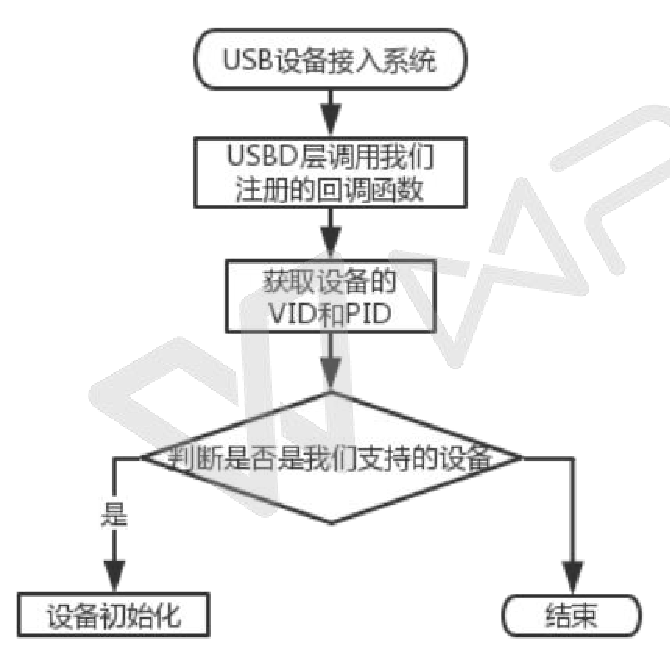
\includegraphics[width=.9\textwidth]{./graphics/device-recognize.pdf}
\caption{设备识别流程图}\label{fig:device-recognize}
\end{figure}

\begin{table}[!h]
\centering
\begin{tabular}{|c|c|c|c|c|c|c|}
\hline
{\hei{PID}}&{0x045B}&{0x0471}&{0x0489}&{0x0489}&{0x10C4}&{0x10C4}\\ 
\hline
{\hei{VID}}&{0x0053}&{0x066A}&{0xE000}&{0xE003}&{0x80F6}&{0x8115}\\
\hline 
{\hei{PID}}&{0x10C4}&{0x10C4}&{0x10C4}&{0x10C4}&{0x10C4}&{0x2405}\\
\hline
{\hei{VID}}&{0xEA60}&{0x813D}&{0x813F}&{0x814A}&{0x814B}&{0x0003}\\
\hline
\end{tabular}
\caption{目前支持的设备列表}\label{tab:目前支持的设备列表}
\end{table}


\subsubsection{驱动缓冲的实现}
	在驱动的内部我们会建立一个循环缓冲区来接收上层程序写入、从设备接收的数据,若系统中没有USB口转串口的设备,那么所有的上层应用往外输出的数据就只会写入到该循环缓冲区当中,当循环缓冲区中的数据已经满了之后,遵循先进先出的原则来覆盖数据。当USB口转串口设备连接上时,若循环缓冲区当中已经有数据存在,则会立即启动发送数据的过程,若没有数据,则什么也不做。
	
	在每一个设备初始化的时候我们都会为该设备分配读缓存和写缓存,缓存空间的大小作为以宏的方式定义在头文件当中,方便以后改动,分别定义为:WRITE_BUFFER_SIZE、READ_BUFFER_SIZE。
	由于计算机的内存是线性地址空间,因此环形缓冲区需要特别的设计才能够从逻辑上实现,通常环形缓冲区需要4个指针:
	 \begin{itemize}
	 \item 在内存中实际开始位置的指针;
	 \item 在内存中实际结束位置的指针,或者缓冲区的长度;
	 \item 存储在缓冲区中的有效数据的开始位置(读指针);
	 \item 存储在缓冲区中的有效数据的结束位置的指针(写指针)。
	 \end{itemize}


通过比较我们选择第三种范式方式作为我们底层驱动中缓冲区空/满的判断方式,同时我们会将缓冲区的大小设置成2的幂,这样我们就可以不需要镜像指示位和取余操作,只需要通过简单的条件表达式就可以判断缓冲区的空/满,这减少了我们的驱动程序本身的运算量和存储空间的消耗,节省了数据传输过程中的处理时间。


\subsubsection{设备的初始化}

	设备的初始化包括获取该USB设备的各种描述符信息。包括配置描述符信息、接口描述符信息、端点描述符信息。再通过所获得的这些信息来创建到输出端点的管道和对设备进行设置,我们在此处将设备的波特率初始化为115200,数据位为8位,1个停止位,没有奇偶校验,没有流控。设备的初始化流程图如\autoref{fig:device-init}所示。
\begin{figure}[!h]
\centering
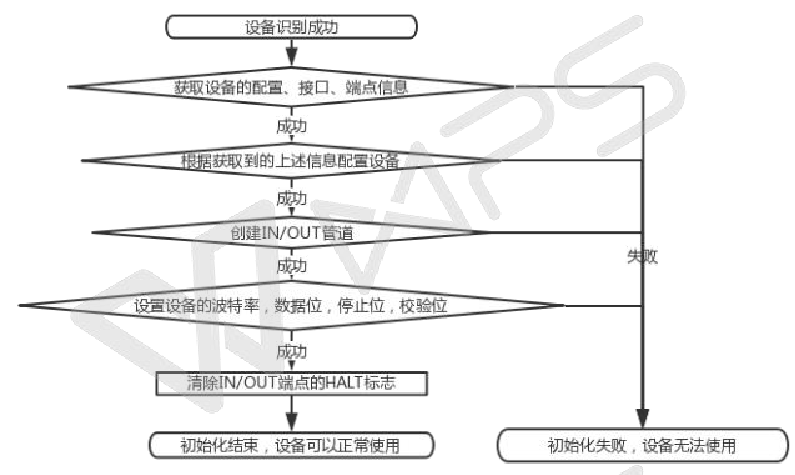
\includegraphics[width=1.0\textwidth]{./graphics/Dev-Init.pdf}
\caption{设备初始化流程图}\label{fig:device-init}
\end{figure}

这些描述符同样是通过usbdDescriptorGet()函数来发送设备的标准描述符命令来获取,在获取到
这些信息之后,通过usbdConfigurationSet()、usbdInterfaceSet()来配置设备,通过usbdPipeCreate()函数来设置设备的输入、输出管道,通过管道来连接设备的输入、输出端点。部分关键代码如下:
\lstset{language=C}
\begin{lstlisting}
...  
  usbdDescriptorGet (cp210xHandle, pCp210xDev->nodeId,USB_RT_STANDARD | USB_RT_DEVICE, USB_DESCR_CONFIGURATION,0, 0, USB_MAX_DESCR_LEN, pBfr, &actLen) 
  pCfgDescr = usbDescrParse (pBfr, actLen,USB_DESCR_CONFIGURATION)
  pScratchBfr = pBfr;
  ifNo = 0;
  while ((pIfDescr = usbDescrParseSkip (&pScratchBfr,&actLen,USB_DESCR_INTERFACE))!= NULL){
    if (ifNo == pCp210xDev->interface)
		break;
	ifNo++;
  }
  pOutEp = findEndpoint(pScratchBfr, actLen, USB_ENDPOINT_OUT)
  pInEp = findEndpoint(pScratchBfr,actLen,USB_ENDPOINT_IN))
...  
  usbdConfigurationSet (cp210xHandle, pCp210xDev->nodeId,pCfgDescr->configurationValue,pCfgDescr->maxPower * USB_POWER_MA_PER_UNIT)
...  
  usbdInterfaceSet(cp210xHandle,pCp210xDev->nodeId,pCp210xDev->interface,pIfDescr->alternateSetting);
...  
  usbdPipeCreate(cp210xHandle,pCp210xDev->nodeId,pOutEp->endpointAddress,pCfgDescr->configurationValue,pCp210xDev->interface,USB_XFRTYPE_BULK,USB_DIR_OUT,maxPacketSizeOut,0,0,&pCp210xDev->outPipeHandle)
...  
  usbdPipeCreate(cp210xHandle,pCp210xDev->nodeId,pInEp->endpointAddress,pCfgDescr->configurationValue,pCp210xDev->interface,USB_XFRTYPE_BULK,USB_DIR_IN,maxPacketSizeIn,0,0,&pCp210xDev->inPipeHandle)
...
\end{lstlisting}


\subsubsection{设备打开/关闭函数}

	用户在使用一个设备之前必须先打开这个设备,底层驱动响应函数中根据设备的需要将进行中断注册和使能设备工作配置等操作。对于我们的USB口转串口驱动而言,我们不需要自己管理中断,USBD层会为我们进行中断的管理工作,而配置工作我们在设备的初始化工作中已经完成,因此此处我们的设备打开工作,只需要简单的记录设备被打开的次数,并返回一个文件描述符即可。代码如下所示:
	
\lstset{language=C}
\begin{lstlisting}
LOCAL CP210X_DEV * cp210xDevOpen(DEV_HDR *pDevHdr, char *name, int flags,int mode)
{
	CP210X_DEV *pCp210xDev;
	pCp210xDev = (CP210X_DEV *)pDevHdr;
	(pCp210xDev->numOpen)++;
	return (pCp210xDev);
}
\end{lstlisting}

	需要注意的是第一个参数是由 IO 子系统提供的,IO 子系统在根据驱动号寻址到对应驱动函数时,其将系统设备列表中存储的设备结构作为第一个参数调用 cp210xDevOpen。实际上该参数是一个 CP210X\_ DEV 结构类型,但是 IO 子系统只认识DEV\_ HDR 结构。所以在 cp210xDevOpen函数中我们需要首先将这个 DEV\_ HDR 结构转换成 SPI\_ DEV,这基本上是所有底层驱动函数实现中第一条语句需要完成的任务。当然,驱动程序员也可以直接将第一个参数的类型设置为自定义结构类型,那么对于我们USB口转串口驱动,以上  cp210xDevOpen 函数的调用原型就变为:LOCAL int cp210xDevOpen(CP210X\_ DEV *pCp210xDev, char *name, int flags,int mode)这并不会造成什么影响,因为 IO 子系统传递过来实际上就是 CP210X\_ DEV 结构类型,只不过 IO 子系统对于驱动自定义参数并不关心,其只需要对 DEV\_ HDR 进行操作就可满足 IO 子系统本身管理的需要,其他自定义参数完全由底层驱动本身进行解释和使用。
	
	第二个参数是设备名匹配后的剩余部分,在我们的应用中,由于 open 函数调用时输入的路径名与系统设备列表中的设备名完全匹配,故此处的 name 应为空字符串。但是对于在文件系统层下的块设备而言,此处 name 指向的就是块设备节点名后的子目录和文件名。

	第三,四个参数就是用户 open 调用时传入的第二,三个参数,IO 子系统原封不动的将他们传递给了 cp210xDevOpen 函数。
	
	返回值为CP210X\_ DEV结构类型,一般返回如下两种值:一个有效的CP210X\_ DEV结构指针表示 cp210xDevOpen 调用成功,ERROR 则表示 cp210xDevOpen 调用失败,IO 子系统根据有效指针或者ERROR 返回一个文件描述符或者返回错误。cp210xDevOpen 函数的返回值非常重要,这个指针将被 IO 子系统保存,用于其后对驱动中读写,控制函数的调用。这个返回的指针将作为这些函数的第一个参数。
	
	设备的关闭和设备的打开操作是相反的操作,在关闭操作当中我们只需要对设备记录的打开次数进行减法操作即可。

\subsubsection{设备的读写}
	在成功打开一个设备后,用户程序将得到一个文件描述符,此后用户就可以使用这个文件描述符对设备进行读写,控制操作。底层驱动读写函数原型如下。

\lstset{language=C}
\begin{lstlisting}
LOCAL int cp210xDevWrite(CP210X_DEV *pCp210xDev, char *buffer,UINT32 nBytes)
LOCAL int cp210xDevRead(CP210X_DEV *pCp210xDev, char *buffer,UINT32 nBytes)
\end{lstlisting}

此处我们将这两个函数的第一个参数类型直接设置为 CP210X\_ DEV 结构类型而不是DEV\_ HDR,只是为了向大家展示两种方式都是允许的,在我们的实际编程中应该一种方式一以贯之。cp210xDevWrite,cp210xDevRead函数的第一个参数是实际上是cp210xDevOpen 函数的返回值。

由于我们的驱动程序的初始化方式比较特殊,所以此处对数据的输出操作的流程也需要有相应的改变。在驱动程序中我们设置了一个4K的数据缓冲区来接收数据,设备的初始化之后就先查询缓冲区中是否存在数据,若存在数据则将其发送,若不存在则等待其他程序调用write写入数据来触发数据的发送操作,系统调用write()在该驱动程序中对应的函数为cp210xDevWrite()函数,这个函数会接受write()发送过来的数据,并将其存入缓冲区中,并判断是否需要触发数据的发送操作。发送数据的触发操作只会在当前没有数据在发送时完成,若调用write时设备已经在发送数据,则只是将write的数据存入缓冲区,设备发送完当前正在发送的数据之后会去判断缓冲区中是否还有数据,有数据则会继续发送。其流程图如\autoref{fig:outData-diagram} 所示。

\begin{figure}[!h]
\centering
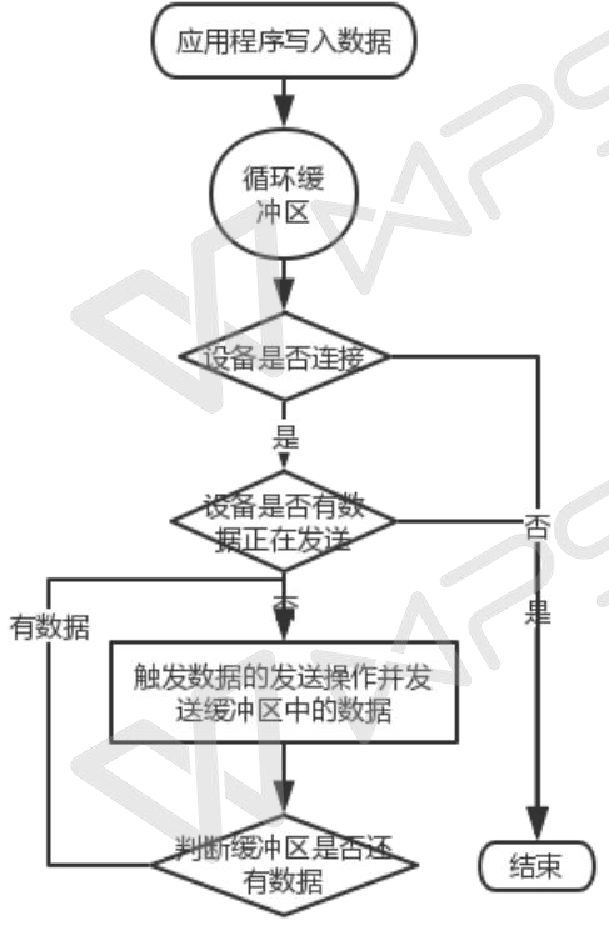
\includegraphics[width=.7\textwidth]{./graphics/data-send-diagram.pdf}
\caption{数据发送逻辑图}\label{fig:outData-diagram}
\end{figure}


cp210xDevRead 和 cp210xDevWrite 的实现非常相似,只是更换了一下数据的传输方向。cp210xDevRead在底层也有一个循环缓冲区用来接收从USB口转串口设备发送来的数据,当需要读取 nbytes 个字节而缓冲区内的字节不够时,read就会阻塞,直到USBD层通知你有新的数据到来时才会继续进行读操作。同时也在驱动中启动了一个计时器,如果在计时器时间到了之后,还未能满足需要读取的字节数,则退出本次读写操作,返回当前已处理的字节数。


\subsubsection{设备的控制操作}
	设备控制简单的说用户对于设备某些工作行为的再配置。基于设备的类型,这些由驱动和 IO 子系统提供给用户的再配置参数会有所差别。Vxworks(其他通用操作系统也是如此)对各种类型的设备都抽取了一组共同属性作为配置选项,如串口波特率再配置就是一个串口标准属性。事实上,虽然有所约定,底层驱动完成可以虽然有所约定,底层驱动完成可以按照自己的标准对这些再配置属性进行选择:可以选择只实现其中某些再配置参数,可以按照特定设备的特殊情况选择对某个再配
置选项的响应方式或者转移再配置参数等等。可以说,设备控制函数既提供给了用户控制设备的方便性,也对底层设备的实现提供了极大的方便性,当然,底层驱动程序员不可以“欺骗”用户,必须完成用户要求的基本配置要求方可根据需要在做一些辅助性的配置工作,这是底层驱动设备控制实现函数的基本原则。

	除了 Vxworks 操作系统本身提供的控制参数外,对于一个特定设备也有自己的特定参数,这些也可以作为选项提供给用户进行控制。一般而言,底层驱动需要定义一个头文件,将设备特定参数在其中进行定义,而后将这个头文件提供给用户程序,当用户对设备进行操作时,其包含这个头文件,使用其中定义的特定参数对设备进行控制。IO 子系统实际上不加任何
改变的将用户使用的选项参数或者控制命令传递给了底层驱动,由底层驱动完成对选项参数或控制命令的解释和使用。
设备控制函数原型如下:
\lstset{language=C}
\begin{lstlisting}
LOCAL int cp210xDevIoctl(CP210X_DEV *pCp210xDev, int request, void *someArg )
\end{lstlisting}

对于我们的 USB口转串口驱动,在实际使用中,再配置参数和命令有很多,但是目前我们只提供设备的波特率、数据位、校验位、流控的参数和命令。这些控制对于普通的USB设备而言是没有的,他们在定义上属于USB的厂商自定义请求,在VxWorks中使用usbdVendorSpecific()函数来发送USB的厂商自定义请求,该函数的原型如下:
\lstset{language=C}
\begin{lstlisting}
STATUS usbdVendorSpecific
(
  USBD_CLIENT_HANDLE clientHandle,/* Client handle */
  USBD_NODE_ID nodeId,	/* Node Id of device/hub */
  UINT8 requestType,	/* bmRequestType in USB spec. */
  UINT8 request,		/* bRequest in USB spec. */
  UINT16 value,			/* wValue in USB spec. */
  UINT16 index,			/* wIndex in USB spec. */
  UINT16 length,		/* wLength in USB spec. */
  pUINT8 pBfr,			/* ptr to data buffer */
  pUINT16 pActLen		/* actual length of IN */
)
\end{lstlisting}
其中第二个参数是请求类型,表示该类型是从主机到设备的,还是从设备到主机的,有四种类型,分别是REQTYPE\_ HOST\_ TO\_ INTERFACE(0x41),REQTYPE\_ INTERFACE\_ TO\_ HOST(0xC1),REQTYPE\_ HOST\_ TO\_ DEVICE(0x40),REQTYPE\_ DEVICE\_ TO\_ HOST((0xC0)),第三个参数是具体的请求,对于我们的设备而言能响应的部分主要请求如\autoref{tab:厂商指定请求}所示。

\begin{table}[!h]
\centering
\begin{tabular}{|c|c|c|c|}
\hline
{\hei{宏名}}&{\hei{代码}}&{\hei{宏名}}&{\hei{代码}}\\
\hline
{CP210X\_ IFC\_ ENABLE}&{0x00}&{CP210X\_ SET\_ BAUDDIV}&{0x01}\\
\hline
{CP210X\_ GET\_ BAUDDIV}&{0x02}&{CP210X\_ SET\_ LINE\_ CTL}&{0x03}\\
\hline
{CP210X\_ GET\_ LINE\_ CTL}&{0x04}&{CP210X\_ SET\_ BREAK}&{0x05}\\
\hline
{CP210X\_ IMM\_ CHAR}&{0x06}&{CP210X\_ SET\_ MHS}&{0x07}\\
\hline
{CP210X\_ SET\_ XOFF}&{0x0A}&{CP210X\_ SET\_ XON}&{0x09}\\
\hline
{CP210X\_ SET\_ FLOW}& 0x13 & CP210X\_ GET\_ FLOW & 0x14\\
\hline
CP210X\_ EMBED\_ EVENTS	& 0x15 & CP210X\_ GET\_ EVENTSTATE & 0x16\\
\hline
CP210X\_ SET\_ CHARS & 0x19 & CP210X\_ GET\_ BAUDRATE & 0x1D\\
\hline
CP210X\_ SET\_ BAUDRATE & 0x1E & CP210X\_ VENDOR\_ SPECIFIC & 0xFF\\
\hline
\end{tabular}
\caption{厂商指定请求}\label{tab:厂商指定请求}
\end{table}

\subsubsection{驱动卸载}
	在驱动的初始化中我们使用 iosDrvInstall 函数向 IO 子系统注册了我们的驱动,同时 IO 子系统也提供了另外一个相反作用的函数注销我们的驱动,这个函数就是 iosDrvRemove。该函数调用原型如下 :
\lstset{language=C}
\begin{lstlisting}
STATUS iosDrvRemove 
 ( 
 int drvnum, /* driver to remove, returned by iosDrvInstall()*/ 
 BOOL forceClose /* if TRUE, force closure of open files */ 
); 
\end{lstlisting}

该函数的第二个参数指定是否强制进行卸载,并将所有与此驱动有关的文件描述符关闭。如果强制关闭,则 IO 子系统将遍历系统文件描述符表,检查每个描述符对应结构中的驱动号是否等于要卸载驱动的驱动号,如果相同,则调用这个驱动的 close 实现函数进行关闭,同时释放文件描述符表中该表项,此时用户层的文件句柄将自动失去功效,如果用户其后使用这个文件描述符,将直接得到一个错误返回。

除了驱动卸载函数之外,我们的驱动初始化时还向USBD层进行了注册,在卸载的时候也应该注销USBD层的注册,同时注销动态注册的回调函数并从系统的设备表当中删除掉该设备。之后还应该对该驱动占用的所有其他的系统资源进行释放。

至此,我们已经完成了该特定需求下的USB口转串口驱动程序的所有组成部分的设计和实现。

\subsection{通用多设备驱动的实现}
多设备支持的驱动程序在初始化的时候与特定需求单设备支持的驱动初始化的过程是不一样的,需要支持多设备,首先需要在识别设备后给每一个设备分配一个设备名,并加入到系统设备表当中,然后需要给每一个设备初始化自己的设备结构体多设备下的驱动运行流程如\autoref{fig:MDev-Drv-diagram}所示。

\begin{figure}[p, !h]
\centering
  \begin{subfigure}[b]{1.0\textwidth}
  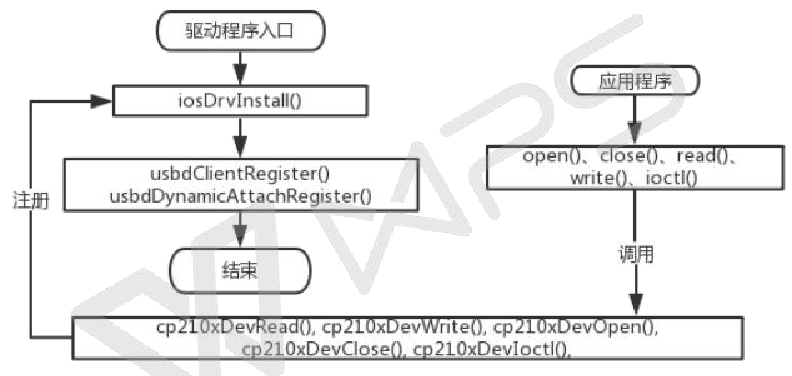
\includegraphics[width=\textwidth]{./graphics/MDev-Drv-Diagram-a.pdf}
  \caption{}\label{fig:MDevice-Driver-diagram-a}
  \end{subfigure}
  ~
  \begin{subfigure}[b]{1.0\textwidth}
  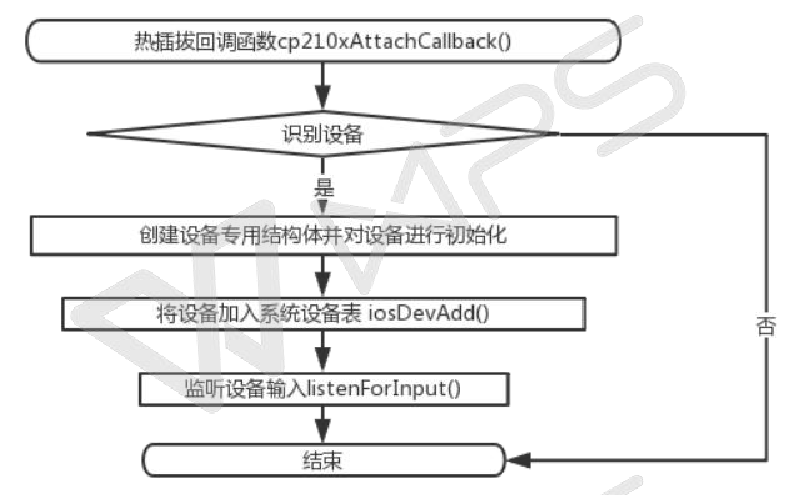
\includegraphics[width=\textwidth]{./graphics/MDev-Drv-Diagram-b.pdf}
  \caption{}\label{fig:MDevice-Driver-diagram-b}
  \end{subfigure}
\caption{多设备驱动运行流程图}\label{fig:MDev-Drv-diagram}
\end{figure}


与特定需求单设备的驱动相比,这里驱动程序的变化主要在驱动的初始化和读写函数部分,同时设备自定义的数据结构会更加复杂,需要保存更多与具体的设备相关的信息。

\subsubsection{设备的自定义结构体}
多设备的驱动自定义结构体的定义如下所示:
\lstset{language=C}
\begin{lstlisting}
typedef struct cp210x_dev
{
  DEV_HDR cp210xDevHdr; /*must be first field*/
  LINK 	devHdrLink; /*linked list of  devhdr structs*/
  UINT16 numOpen;
  USBD_NODE_ID nodeId; /*device nodeID*/
  UINT16 configuration; 
  UINT16 interface; /*a interface of this device*/
  UINT16 interfaceAltSetting;
  UINT16 vendorId;
  UINT16 productId;
  BOOL connected;
  
  int trans_len;
  USBD_PIPE_HANDLE outPipeHandle; /* USBD pipe handle for bulk OUT pipe*/
  USB_IRP	outIrp; /*IRP to monitor output to device*/
  BOOL outIrpInUse;
  UINT32 outErrors; /*TRUE while IRP is outstanding*/
  UINT8 trans_buf[64];
  UINT16  outEpAddr;  
  
  USBD_PIPE_HANDLE inPipeHandle;
  USB_IRP inIrp;
  BOOL inIrpInUse;
  UINT8 inBuf[64];
  UINT32 inErrors;
  UINT16 inEpAddr;
  
  char *writeBuf;
  int writeFront;
  int writeRear;
  char *readBuf;
  int readFront;
  int readRear;
} CP210X_DEV, *pCP210XDEV;
\end{lstlisting}
	在这个结构体当中我们增加了每个设备的读写缓冲区的指针和各个缓冲区的头尾指针。同时使用了一个链表devHdrLink来链接在系统上的由该驱动支持的设备,每次检测到新设备时我们可以通过将新添加的设备增加到这个链表当中,之后可以通过nodeId来从多个设备中定位我们的设备是否存在,之后我们可以给每一个设备分配一个设备名。部分代码如下所示:
\lstset{language=C}
\begin{lstlisting}
...
 usbListLinkProt(&devListHdr,(pVOID)pCp210xDev,(pLINK)&pCp210xDev->devHdrLink,LINK_TAIL,cp210xMutex);
...

LOCAL pCP210XDEV findDevHdr(USBD_NODE_ID nodeId)
{
	pCP210XDEV pCp210xDev =  usbListFirst(&devListHdr);

	while(pCp210xDev != NULL)
	{
		if(pCp210xDev->nodeId == nodeId)
			break;
		pCp210xDev = usbListNext(&pCp210xDev->devHdrLink);
	}
	return pCp210xDev;
}
\end{lstlisting}

\subsubsection{驱动注册和设备创建}

	比较单设备驱动初始化(如\autoref{fig:SDevice-Driver-diagram-a}所示)和多设备驱动初始化(如\autoref{fig:MDevice-Driver-diagram-a}所示),我们可以看出在驱动注册过程中两者的区别,在单设备驱动的初始化中我们先完成设备结构体的创建并定好一个设备名,之后直接将其加入到系统的设备表当中,即使此时没有设备连接。而在多设备的驱动初始化当中我们是在驱动的回调函数中驱动识别完了设备之后再完成设备结构体的创建和加入系统设备表的,这种方式是通用的设备驱动常采用的方式。
	在设备创建时我们会通过判断已连接设备的个数来决定当前设备所采用的设备名,部分代码如下:

\lstset{language=C}
\begin{lstlisting}
LOCAL int getCp210xDeviceNum(CP210X_DEV *pCp210xDev)
{
...
  for (int index=0; index < CP210X_MAX_DEVICE; index++)
    if (pCp210xDevArray[index] == NULL){
      pCp210xDevArray[index] = pCp210xDev;
      return (index);
    }
...
}
	
LOCAL STATUS cp210xAttachCallback(USBD_NODE_ID nodeId, UINT16 attachAction,UINT16 configuration,UINT16 interface,UINT16 deviceClass,UINT16 deviceSubClass, UINT16 deviceProtocol)
{
  ...
  cp210xUnitNum = getCp210xDeviceNum(pCp210xDev);
  sprintf (cp210xName, "%s%d", CP210X_NAME,cp210xUnitNum);
  if(iosDevAdd(&pCp210xDev->cp210xDevHdr,cp210xName,cp210xDrvNum) != OK)
  ...
}
\end{lstlisting}

\subsubsection{设备读写}
	对于通用多设备的写操作,与设定设备的操作不同的是设备连接上时,没有一个自动发送缓冲区的数据的过程,此时设备没有连接上也不可能往缓冲区中写入数据。其基本流程如下:	
	
	\begin{enumerate}
	\item 将数据拷贝到输出循环缓冲区当中,若缓冲区已满则等待。
	\item 判断设备是否仍然处于连接状态。
	\item 若处于连接状态,那么是否有数据正在发送当中。若有数据正在发送,则等待。
	\item 若没有数据在发送,则触发发送数据的操作。
	\item 返回发送的字节数。
	\end{enumerate}
	
	对于数据发送的逻辑控制,使用了VxWoks的同步和互斥信号量。首先在写入数据的时候需要进行互斥写,因为此时设备有可能正在从缓冲区当中取数据进行输出操作,那么这是写入输出缓冲区就需要等待,否则可能会造成缓冲区的混乱,造成输出结果与输入数据不一致。当设备输出从缓冲区拷贝完成之后就会释放互斥信号量,此时写入操作就可以往输出缓冲区中写入数据。
	
	
	对于通用多设备的读操作,我们会事先创建好一个用来读取数据的USB IRP在这个IRP中我们注册一个回调函数,USB的中断会由USBD层来替我们进行管理,当有数据到来时USBD层会调用我们注册的回调函数来通知我们。在驱动程序初始化完成之后我们就会启动listenForInput()这个函数来注册一个USBD的通知过程,一个接收IRP使用完成之后,我们需要重新注册一次,因为每一次的IRP都是单次有效的,所以在cp210xIrpCallback()中我们接受完这一次的IRP的数据之后, 需要新建另一个IRP重新启动下一次的listenForInput()过程。部分关键代码如下:
\lstset{language=C}
\begin{lstlisting}

LOCAL STATUS listenForInput(CP210X_DEV *pCp210xDev)
{
..
  pIrp->userPtr = pCp210xDev;
  pIrp->userCallback = cp210xIrpCallback;
  pIrp->timeout = USB_TIMEOUT_NONE;
  pIrp->transferLen = 64;
  if(usbdTransfer (cp210xHandle, pCp210xDev->inPipeHandle, pIrp) != OK)
...
}

LOCAL void cp210xIrpCallback(pVOID p)
{
...
	if(pIrp == &pCp210xDev->inIrp && pCp210xDev->connected == TRUE)
	{
		if(pIrp->result == OK)
			copy_to_readBuf(pCp210xDev);
			
		if (pIrp->result != S_usbHcdLib_IRP_CANCELED)
			listenForInput(pCp210xDev);
	}
}

\end{lstlisting}




其他的部分如设备的控制、设备打开/关闭、设备卸载函数与单设备下的相比不需要做改变即可完成,此时操作的设备就是我们使用设备名打开的那个设备,IO子系统会将设备名映射到该设备所对应地驱动。









\section{小结}
	本章首先介绍了我们的USB口转串口驱动的设计想法,包括USB口转串口所使用转换器的选择,驱动程序所需要实现的模块,每个模块的功能是什么。接下来对所选择的转换器CP2102的开发进行了介绍,对VxWorks中USB的开发进行了介绍,最后根据我们的设计方案对驱动程序的每一个部分进行了实现。



